\chapter{Pilha (\texttt{stack})}
\label{cap:stack}

\section{Especificação}

O bloco \texttt{stack} tem oito registradores de 11 bits, que guardam os endereços de retorno do contador de programa \cite{tp2}. As operações acontecem na borda de subida do clock:

\begin{itemize}
  \item \textbf{\textit{push}} (\texttt{stack\_push = '1'}): o valor de \texttt{stack\_in} é escrito no primeiro registrador (o topo); ao mesmo tempo, o segundo recebe o conteúdo do primeiro, e assim por diante até o oitavo, que recebe o conteúdo do sétimo;
  \item \textbf{\textit{pop}} (\texttt{stack\_pop = '1'}): o segundo registrador é transferido para o primeiro, o terceiro para o segundo, e assim por diante até o sétimo, que recebe o oitavo; este recebe zero;
  \item \textbf{prioridade}: se \texttt{stack\_push} e \texttt{stack\_pop} estiverem ativos ao mesmo tempo, o \textit{push} tem preferência;
  \item \textbf{reset}: \texttt{nrst} (ativo em nível baixo) zera todos os bits dos oito registradores, de modo assíncrono, e tem preferência sobre todas as outras entradas.
\end{itemize}

Os valores são recuperados em ordem inversa à da escrita (LIFO), e mais de oito \textit{pushes} seguidos fazem o conteúdo mais antigo se perder (\textit{stack overflow}). A saída \texttt{stack\_out} é o primeiro registrador e está sempre ativa. A Figura~\ref{fig:bloco-stack} mostra o diagrama de blocos e o Quadro~\ref{quad:portas-stack} descreve as portas.

\begin{figure}[htb]
\caption{Diagrama de blocos da pilha.}\label{fig:bloco-stack}
\centering
\begin{tikzpicture}[>={Stealth[length=2mm]}]
  \renewcommand{\fio}{1.4}
  \node[draw, minimum width=3.2cm, minimum height=4cm, font=\large\bfseries] (bloco) {stack};
  \pentrada{1.6}{nrst}{}
  \pentrada{0.8}{clk\_in}{}
  \pentrada{0}{stack\_in[10..0]}{line width=1.2pt}
  \pentrada{-0.8}{stack\_push}{}
  \pentrada{-1.6}{stack\_pop}{}
  \psaida{0}{stack\_out[10..0]}{line width=1.2pt}
\end{tikzpicture}
\fonte{Elaborada pelos autores, com base em \textcite{tp2}.}
\end{figure}

\begin{quadro}[htb]
  \caption{Portas da pilha.}
  \label{quad:portas-stack}
  \centering
  \begin{tabular}{lcp{9cm}}
    \hline
    Porta & Direção & Descrição \\ \hline
    \texttt{nrst} & entrada & \textit{Reset} assíncrono, ativo em nível baixo; zera as oito posições \\
    \texttt{clk\_in} & entrada & Clock; \textit{push} e \textit{pop} acontecem na borda de subida \\
    \texttt{stack\_in[10..0]} & entrada & Valor a ser empilhado \\
    \texttt{stack\_push} & entrada & Habilita o \textit{push}, ativa em nível alto; tem preferência sobre o \textit{pop} \\
    \texttt{stack\_pop} & entrada & Habilita o \textit{pop}, ativa em nível alto \\
    \texttt{stack\_out[10..0]} & saída & Topo da pilha (primeiro registrador), sempre ativo \\ \hline
  \end{tabular}
  \fonte{Adaptado de \textcite{tp2}.}
\end{quadro}

\section{Implementação}

\subsection{Arquitetura}

A pilha é um \textit{array} de oito vetores de 11 bits, em que \texttt{r(0)} é o topo e \texttt{r(7)} é o fundo, e é descrita como um registrador de deslocamento, num único \texttt{process} sensível a \texttt{nrst} e \texttt{clk\_in}:

\begin{itemize}
  \item o reset zera o \textit{array} inteiro com um agregado aninhado;
  \item na borda de subida, um \texttt{IF}/\texttt{ELSIF} testa primeiro \texttt{stack\_push} e depois \texttt{stack\_pop}, o que dá ao \textit{push} a preferência exigida;
  \item o \textit{push} escreve \texttt{stack\_in} em \texttt{r(0)} e desloca \texttt{r(0 TO 6)} para \texttt{r(1 TO 7)}; o \textit{pop} desloca \texttt{r(1 TO 7)} para \texttt{r(0 TO 6)} e zera \texttt{r(7)};
  \item sem \textit{push} nem \textit{pop}, nada é atribuído e todos os registradores mantêm o valor.
\end{itemize}

A saída \texttt{stack\_out <= r(0)} é uma atribuição concorrente.

\subsection{Decisões de projeto}

\begin{itemize}
  \item \textbf{Atribuição por fatias}: as atribuições \texttt{r(1 TO 7) <= r(0 TO 6)} e \texttt{r(0 TO 6) <= r(1 TO 7)} deslocam as oito posições de uma só vez. Como num processo as atribuições de sinais só têm efeito quando ele termina, todas as posições leem o valor \textit{antigo} de seus vizinhos, que é exatamente o comportamento de um registrador de deslocamento; um laço ou variáveis seriam desnecessários.
  \item \textbf{Prioridade do \textit{push}}: é obtida só pela ordem dos testes, sem lógica adicional.
  \item \textbf{Não há contador de ocupação}: o enunciado não pede sinalização de pilha cheia ou vazia, e o \textit{pop} numa pilha vazia apenas entrega zeros, pois o fundo é preenchido com zero a cada deslocamento.
\end{itemize}

\subsection{Circuito em nível RTL}

A Figura~\ref{fig:rtl-stack} mostra a interpretação feita pelo RapidRTL: um único registrador de 88 bits (8 posições de 11 bits), com reset assíncrono e habilitação (\texttt{\$adffe}). A habilitação é o OU de \texttt{stack\_push} e \texttt{stack\_pop} (o \texttt{\$reduce\_bool}), como no diagrama funcional da especificação. A entrada D vem de dois multiplexadores em cascata: o primeiro, controlado por \texttt{stack\_pop}, entrega o deslocamento do \textit{pop} (com zeros no fundo); o segundo, controlado por \texttt{stack\_push}, escolhe entre esse valor e o deslocamento do \textit{push} (com \texttt{stack\_in} na primeira posição). Como o \textit{push} é o último a ser selecionado, ele tem preferência sobre o \textit{pop}. O Quartus aloca 88 \textit{flip-flops} e 89 elementos lógicos.

\begin{figure}[htb]
  \centering
  \caption{Circuito da pilha em nível RTL.}
  \label{fig:rtl-stack}
  \includegraphics[width=\textwidth, height=0.4\textheight, keepaspectratio]{stack_rtl.pdf}
  \fonte{Elaborado a partir do site RapidRTL, com base no arquivo \texttt{project/stack/stack.vhd}.}
\end{figure}

\subsection{Código-fonte}

O Código~\ref{lst:stack} apresenta a entidade e a arquitetura completas, com comentários.

\blocovhdl{Descrição VHDL da pilha.}{lst:stack}{stack}{stack.vhd}

\section{Simulação e resultados}

\subsection{Metodologia}

O projeto tem cinco formas de onda (arquivos \texttt{.vwf} em \texttt{project/stack/}), todas com clock de 20\,ns e reset inicial:

\begin{itemize}
  \item \texttt{stack.vwf}: visão geral, com \textit{pushes}, \textit{pops}, \textit{push} e \textit{pop} simultâneos, ciclo sem operação e \textit{pop} com a pilha vazia;
  \item \texttt{stack\_lifo.vwf}: oito \textit{pushes} (100 a 800) seguidos de nove \textit{pops}, que devolvem os valores em ordem inversa e, no último, zero;
  \item \texttt{stack\_overflow.vwf}: dez \textit{pushes}, dos quais os dois mais antigos se perdem, e dez \textit{pops};
  \item \texttt{stack\_push\_pop.vwf}: \textit{push} e \textit{pop} simultâneos, inclusive com a pilha vazia, e pulsos de \texttt{stack\_push} entre bordas e sobre a borda;
  \item \texttt{stack\_reset.vwf}: reset fora de qualquer borda, reset prevalecendo sobre o \textit{push} e pulso curto de reset.
\end{itemize}

O \textit{testbench} \texttt{extras/stack\_tb.vhd} compara o topo da pilha com um modelo de oito posições a cada ciclo, inclusive em esvaziamentos completos da pilha para expor o conteúdo de todas as posições; em casos direcionados e em 1\,000 ciclos pseudoaleatórios, são 1\,167 comparações, sem nenhuma falha. As tabelas de resultados esperados estão em \texttt{extras/casos\_de\_teste.md}.

\subsection{Casos de teste e resultados}

A Figura~\ref{fig:sim-stack} mostra a simulação de \texttt{stack.vwf} e a Tabela~\ref{tab:caso-stack} traz os valores esperados. Cada linha é um intervalo entre mudanças das entradas, com as saídas do fim do intervalo. As tabelas das demais formas de onda estão no Apêndice~\ref{ap:tabelas}.

\begin{figure}[htb]
  \centering
  \caption{Simulação funcional de \texttt{stack.vwf} (visão geral).}
  \label{fig:sim-stack}
  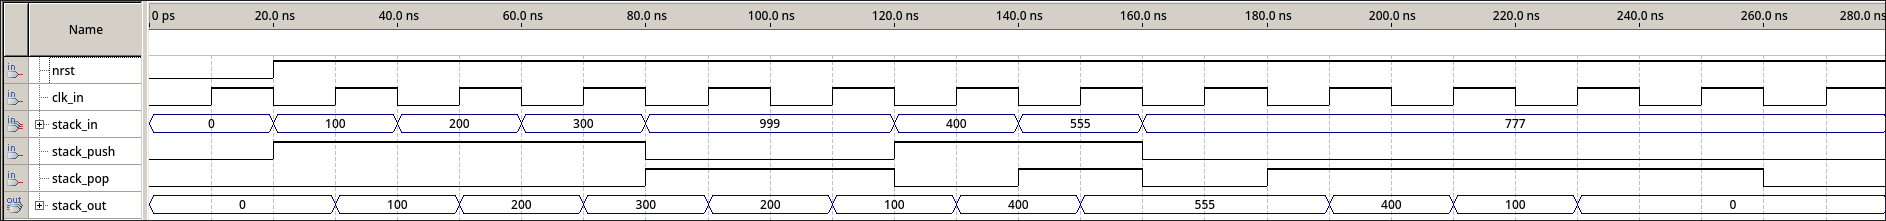
\includegraphics[width=\textwidth]{../../project/stack/stack_simulation.png}
  \fonte{Autoria própria (Quartus II).}
\end{figure}

\Needspace*{12\baselineskip}
{\scriptsize\setlength{\tabcolsep}{3pt}
\begin{longtable}{rcccccp{5.7cm}}
\caption{Casos de teste de \texttt{stack.vwf}: visão geral.}
\label{tab:caso-stack}\\
\hline $t$ (ns) & \texttt{nrst} & \texttt{stack\_in} & \texttt{stack\_push} & \texttt{stack\_pop} & \texttt{stack\_out} & Observação \\ \hline \endfirsthead
\hline $t$ (ns) & \texttt{nrst} & \texttt{stack\_in} & \texttt{stack\_push} & \texttt{stack\_pop} & \texttt{stack\_out} & Observação \\ \hline \endhead
0--20 & 0 & 0 & 0 & 0 & 0 &  \\
20--40 & 1 & 100 & 1 & 0 & 100 & solta o reset; push 100 \\
40--60 & 1 & 200 & 1 & 0 & 200 & push 200 \\
60--80 & 1 & 300 & 1 & 0 & 300 & push 300 \\
80--100 & 1 & 999 & 0 & 1 & 200 & pop (volta a 200) \\
100--120 & 1 & 999 & 0 & 1 & 100 & pop (volta a 100) \\
120--140 & 1 & 400 & 1 & 0 & 400 & push 400 \\
140--160 & 1 & 555 & 1 & 1 & 555 & push e pop juntos: push 555 vence \\
160--180 & 1 & 777 & 0 & 0 & 555 & sem operação (stack\_in muda e é ignorado) \\
180--200 & 1 & 777 & 0 & 1 & 400 & pop (555 sai, volta a 400) \\
200--220 & 1 & 777 & 0 & 1 & 100 & pop (volta a 100) \\
220--240 & 1 & 777 & 0 & 1 & 0 & pop (esvazia, topo = 0) \\
240--260 & 1 & 777 & 0 & 1 & 0 & pop com a pilha vazia: continua 0 \\
260--280 & 1 & 777 & 0 & 0 & 0 & sem operação \\
\hline
\end{longtable}}
\vspace{-0.9cm}
\fonte{Autoria própria. Saídas do fim de cada intervalo, conforme o modelo de referência e a simulação do Quartus II.}


\subsection{Análise dos resultados}

\begin{itemize}
  \item \textbf{\textit{Push}}: os valores 100, 200 e 300 são empilhados nas bordas de 30, 50 e 70\,ns, e o topo acompanha: 100, 200, 300.
  \item \textbf{\textit{Pop}}: nas bordas de 90 e 110\,ns o topo volta a 200 e depois a 100, ou seja, os valores saem na ordem inversa da entrada (LIFO). O valor 999 em \texttt{stack\_in} durante os \textit{pops} é ignorado.
  \item \textbf{Prioridade do \textit{push}}: em 140--160\,ns, \texttt{stack\_push} e \texttt{stack\_pop} estão ativos juntos com \texttt{stack\_in = 555}, e o topo passa a 555; o \textit{pop} seguinte, em 190\,ns, devolve 400, o valor que estava logo abaixo, o que mostra que o 555 foi empilhado e não houve \textit{pop}.
  \item \textbf{Sem operação}: em 160--180\,ns, com as duas entradas em zero, o topo se mantém em 555 mesmo com \texttt{stack\_in = 777}.
  \item \textbf{Pilha vazia}: depois do terceiro \textit{pop} (230\,ns), o topo é 0, e o \textit{pop} extra em 250\,ns continua em 0.
\end{itemize}

As formas de onda adicionais cobrem o que \texttt{stack.vwf} não mostra. Em \texttt{stack\_overflow.vwf}, depois de dez \textit{pushes} os \textit{pops} devolvem 10 a 3 e depois só zeros: os valores 1 e 2 foram perdidos. Em \texttt{stack\_lifo.vwf}, as oito posições, cheias, devolvem 800 a 100 e, no nono \textit{pop}, 0, o que mostra que o \textit{pop} injeta zeros no fundo. Em \texttt{stack\_reset.vwf}, depois do reset assíncrono nada do que foi empilhado antes reaparece.
